\documentclass[tikz,border=8pt]{standalone}
\usepackage{amsmath}
\usetikzlibrary{arrows.meta,positioning,fit,calc}

\begin{document}
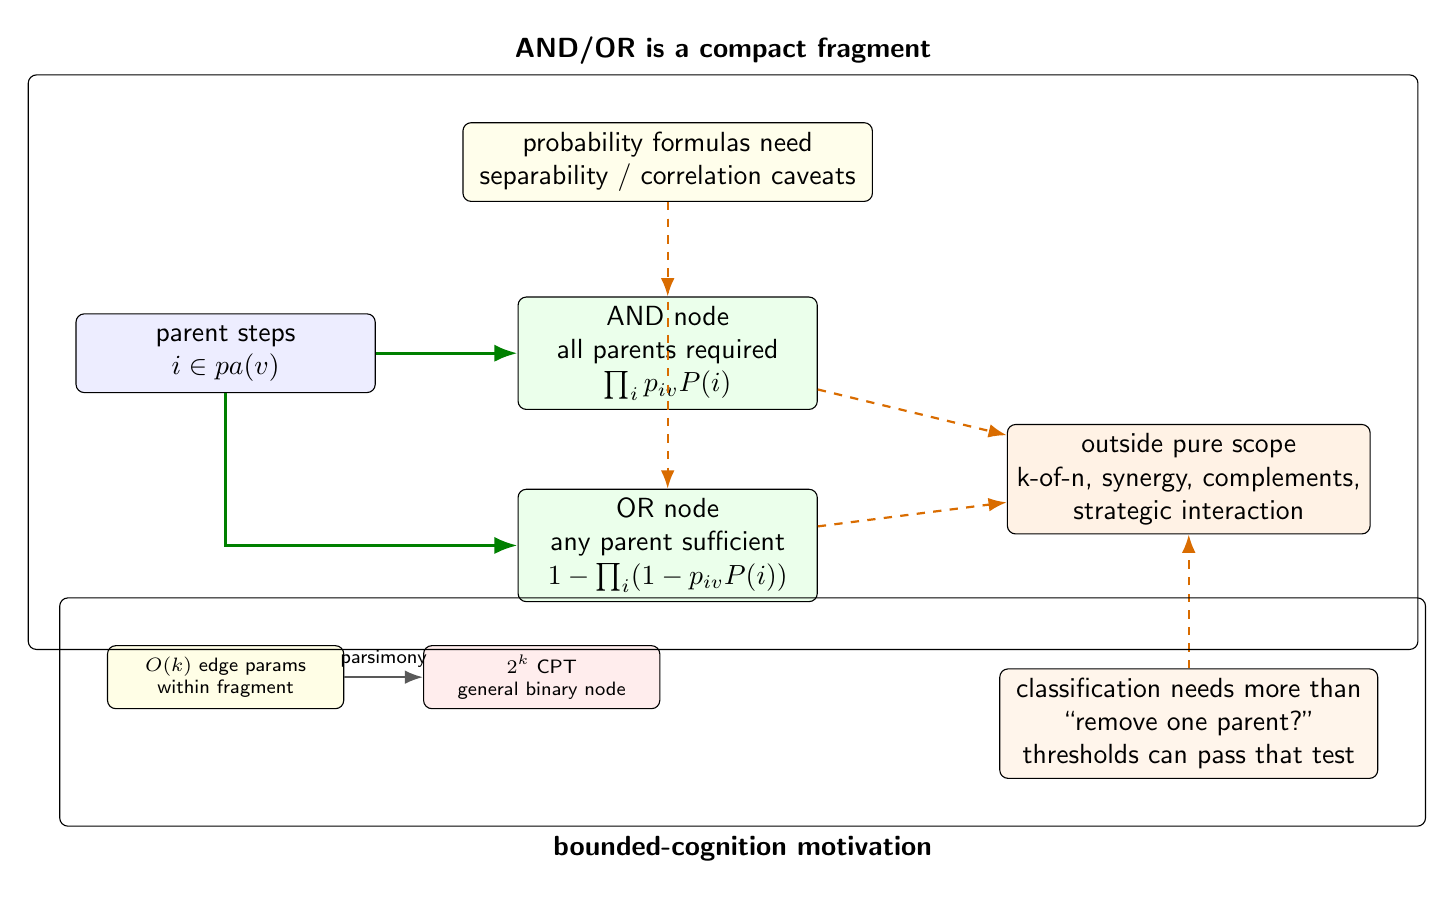
\begin{tikzpicture}[
  font=\sffamily,
  box/.style={draw, rounded corners=3pt, align=center, minimum width=38mm, minimum height=10mm, fill=white},
  small/.style={draw, rounded corners=3pt, align=center, minimum width=30mm, minimum height=8mm, fill=white, font=\sffamily\scriptsize},
  arrow/.style={-Latex, thick, draw=black!65},
  good/.style={-Latex, very thick, draw=green!50!black},
  warn/.style={-Latex, thick, dashed, draw=orange!85!black},
  note/.style={align=center, font=\sffamily\scriptsize}
]

\node[box, fill=blue!7] (parents) {parent steps\\$i\in pa(v)$};
\node[box, right=18mm of parents, fill=green!8] (and) {AND node\\all parents required\\$\prod_i p_{iv}P(i)$};
\node[box, below=10mm of and, fill=green!8] (or) {OR node\\any parent sufficient\\$1-\prod_i(1-p_{iv}P(i))$};
\node[box, right=24mm of and, yshift=-16mm, fill=orange!10] (outside)
  {outside pure scope\\k-of-n, synergy, complements,\\strategic interaction};

\draw[good] (parents) -- (and);
\draw[good] (parents) |- (or);
\draw[warn] (and) -- (outside);
\draw[warn] (or) -- (outside);

\node[small, below=32mm of parents, fill=yellow!10] (cheap) {$O(k)$ edge params\\within fragment};
\node[small, right=10mm of cheap, fill=red!7] (cpt) {$2^k$ CPT\\general binary node};
\draw[arrow] (cheap) -- node[above, note] {parsimony} (cpt);

\node[box, below=17mm of outside, fill=orange!8, minimum width=48mm] (test)
  {classification needs more than\\``remove one parent?''\\thresholds can pass that test};
\draw[warn] (test) -- (outside);

\node[box, above=12mm of and, fill=yellow!8, minimum width=52mm] (corr)
  {probability formulas need\\separability / correlation caveats};
\draw[warn] (corr) -- (and);
\draw[warn] (corr) -- (or);

\node[draw, rounded corners=3pt, fit=(parents)(and)(or)(outside)(corr), inner sep=6mm,
  label={[font=\sffamily\bfseries]above:AND/OR is a compact fragment}] {};
\node[draw, rounded corners=3pt, fit=(cheap)(cpt)(test), inner sep=6mm,
  label={[font=\sffamily\bfseries]below:bounded-cognition motivation}] {};

\end{tikzpicture}
\end{document}
